\documentclass[a4paper,10pt]{article}
\usepackage{graphicx}
\usepackage[english]{babel}
\usepackage{geometry}           
\geometry{letterpaper}                   
\usepackage{graphicx}
\usepackage{amsmath}
\usepackage{amssymb}
\usepackage{subfigure}
\usepackage{wrapfig}
\usepackage{url}
\usepackage[section]{placeins}
\usepackage{fontspec,xltxtra,xunicode}
\title{Three-Dimensional Vizualization and Animation\\Technical Report - Assignment III.}
\author{
  Marfeychuk, Mykhaylo\\
  \texttt{ist194039}
  \and
  Skalický, Matyáš\\
  \texttt{ist194904}
}

\date{} % 31.10.2019

\begin{document}
\maketitle

%\begin{figure}[!htb]
%	\centering
% 	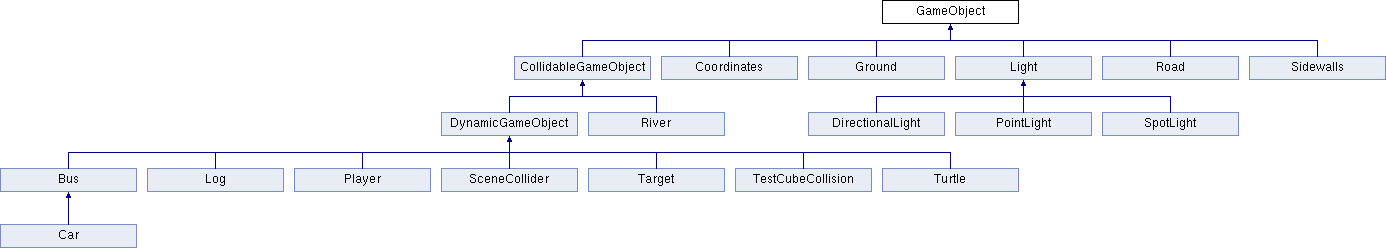
\includegraphics[width=\linewidth]{images/image1.png}
%  	\caption{Objects which inherit from the GameObject class.}
%\end{figure}

\section{Cameras}
The application contains several cameras. The player can switch the camera using the keys 1 to 5. All of the cameras also show information about the game except for the stereo mode, for which we do not show any information on the screen to make the screen less cluttered.

\begin{figure}[!htb]
	\centering
 	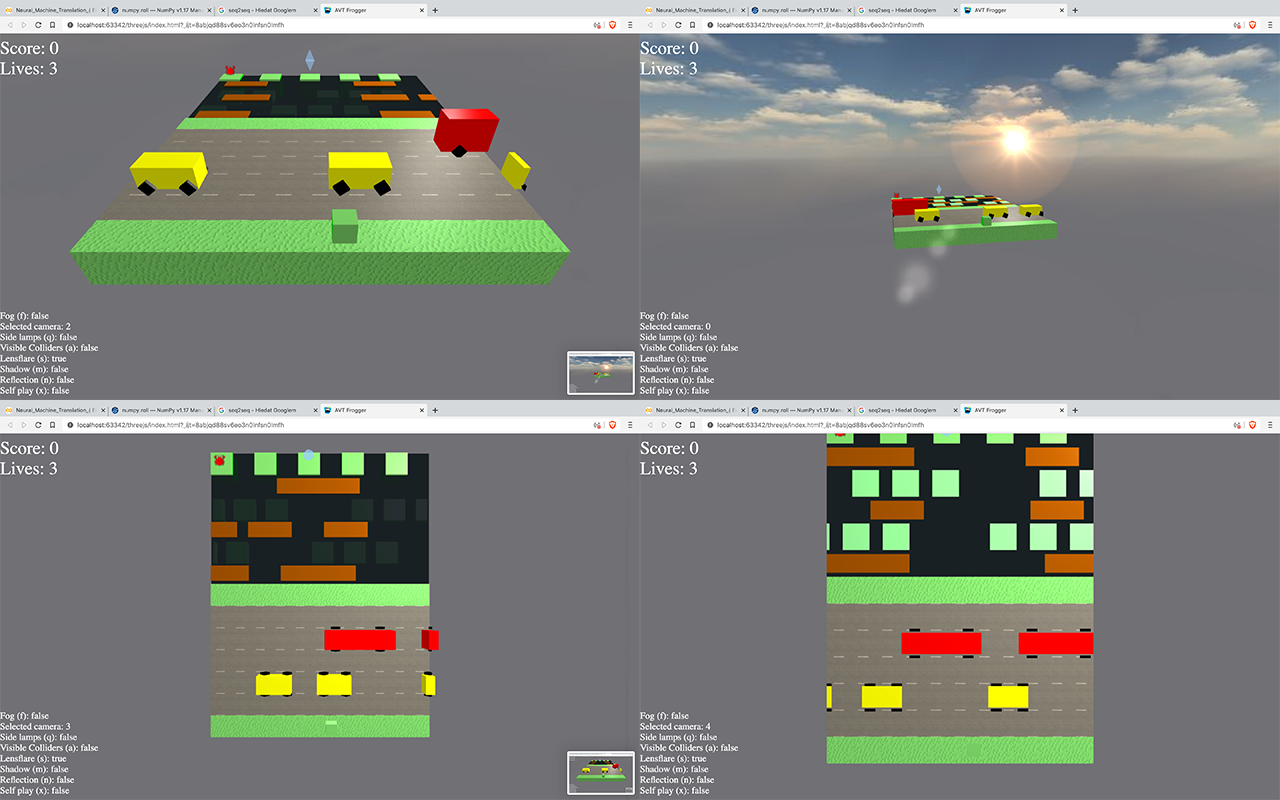
\includegraphics[width=\linewidth]{images/cam_merged.png}
  	\caption{From top left: perspective following camera, rotating perspective camera, top perspective camera and top orthogonal camera.}
\end{figure}

\section{Object movement}

\section{Lights}

\section{Textures}

\section{Collision detection}

\section{Scoring system}

\section{Fog}

\section{Planar reflections}

\section{Planar shadows}

\section{Billboard}

\section{Lens flare}

\section{Shader with Skybox and Environment cube mapping}

\section{Stereo viewing}
The stereo viewing was implemented based on the module provided on the ThreeJS demo accessible at \url{https://threejs.org/examples/webgl_effects_stereo.html}. 

\begin{figure}[!htb]
	\centering
 	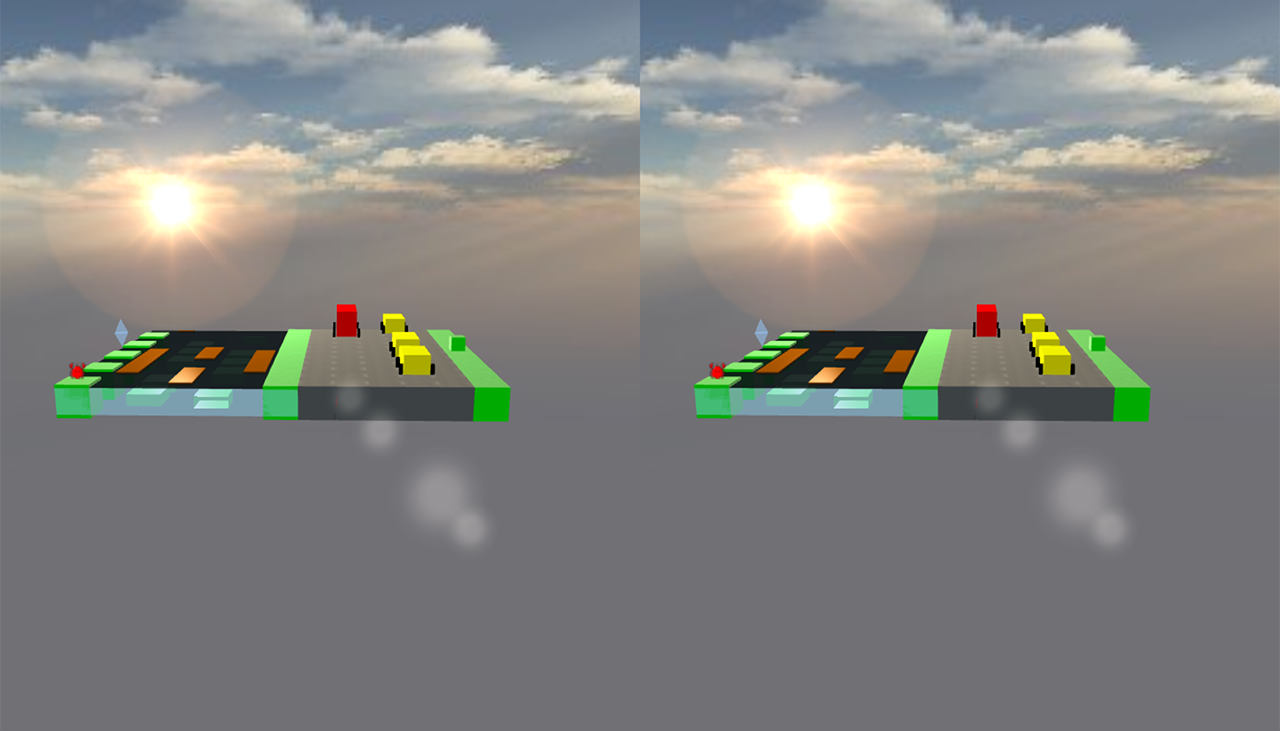
\includegraphics[width=\linewidth]{images/cam_stereo.png}
  	\caption{Stereo perspective rotating camera.}
\end{figure}

\section*{Conclusion}
We have implemented most of the required functionality for the third task of our project. Sadly, due to time contains and also one of our group member missing, we have not implemented the bump-mapping and a particle system. The mobile gyroscope controls were developed, however we ran into a technical problem that the mobile browser is not able to access the gyro data over http and our hosting did not have SSL set up. 

The testing was difficult, since Matyáš's old phone did not run any of the WebGL content, and Mykhaylo's phone was too large to fit into the Google Glass headset. 

\end{document}  